% !TEX root = main.tex

\section{应用层}
应用层协议一般都是采用客户-服务器结构
\begin{center}
\begin{tabular}{|c|c|c|c|}\hline
应用 & 应用层协议 & 传输层协议 & 端口号\\\hline
Email & SMTP [RFC 2821] & TCP & 25\\\hline
远程终端访问 & Telnet [RFC 854] & TCP & -\\\hline
Web & HTTP [RFC 2616] & TCP & -\\\hline
文件传输 & FTP [RFC 959] & TCP & 21\\\hline
域名解析服务 & DNS & UDP & 53\\\hline
简单网络管理协议 & SNMP & UDP & 161\\\hline
\end{tabular}
\end{center}

\subsection{HTTP协议}
\subsubsection{概述}
\begin{itemize}
\item 网页(Web page)是由对象(objects)构成的。这些对象可以是HTML文件、 JPEG图像文件、 MP4视频文件等。
\item 网页的HTML文件中指出了所需的其他对象。
\item 每个对象采用URL指明存放地址。URL由\underline{主机名}和\underline{路径名}构成。
\end{itemize}

HTTP: 超文本传送协议(hypertext transfer protocol),是无状态的(stateless),server不保留过往客户端的任何信息
\begin{itemize}
\item 非持续连接的HTTP:每个时刻最多请求一个Web对象,每建立一个连接最多只能传送一个Web对象。\verb'connection: close'
\item 非流水式持续连接HTTP:每个时刻可以请求多个Web对象,每建立一个连接可以传送多个Web对象。\verb'connection: keep-alive'
\begin{figure}[H]
    \centering
    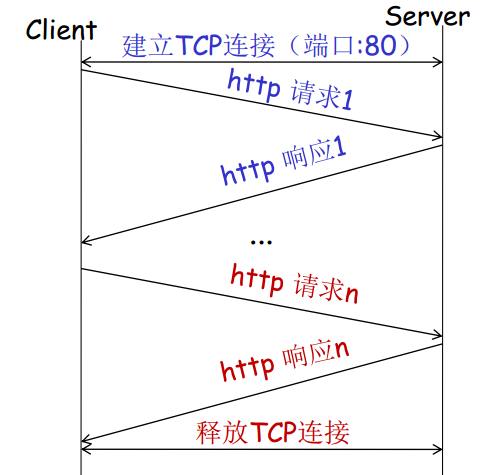
\includegraphics[width=0.4\linewidth]{fig/non-pipelining-http.png}
\end{figure}
\item 流水式持久连接HTTP:可以连续请求多个Web对象,每建立一个TCP连接可以传送多个Web对象。HTTP/1.1 默认使用持续连接。\verb'connection: keep-alive'
\begin{figure}[H]
    \centering
    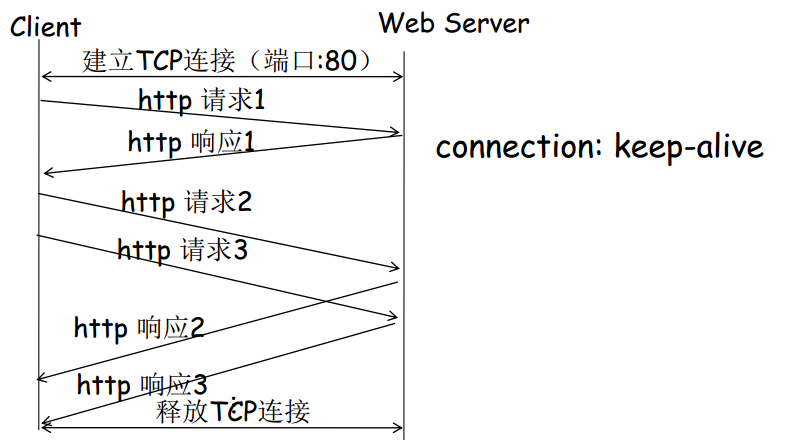
\includegraphics[width=0.6\linewidth]{fig/pipelining-http.png}
\end{figure}
\end{itemize}

\subsubsection{消息}
HTTP请求消息(message)
\begin{figure}[H]
    \centering
    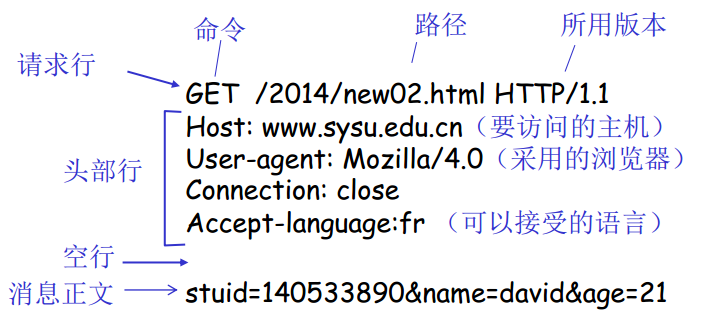
\includegraphics[width=0.6\linewidth]{fig/http-msg.png}
\end{figure}
\begin{itemize}
\item 只有POST命令才有消息正文
\item 每一行均以回车换行结束(\verb'\r\n'),这一点很重要,否则收不到回复!
\end{itemize}

HTTP响应信息
\begin{figure}[H]
    \centering
    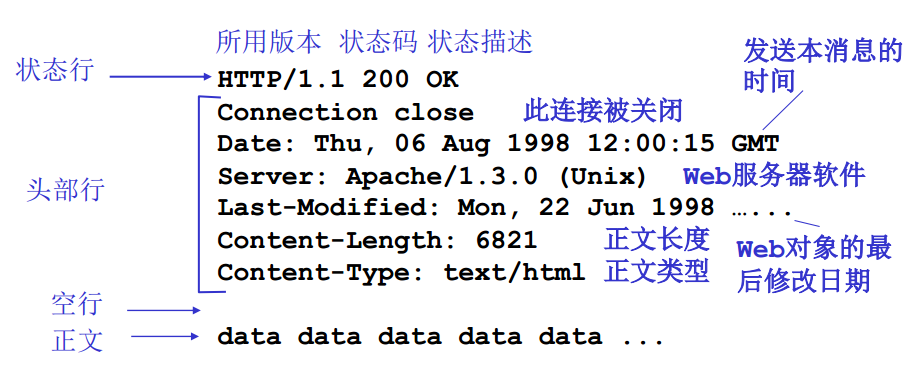
\includegraphics[width=0.6\linewidth]{fig/http-respond.png}
\end{figure}

用telnet建立TCP连接,然后发送GET请求,如
\begin{lstlisting}
telnet www.sysu.edu.cn 80
GET /2012/cn/index.htm HTTP/1.1
Connection: close
Host: www.sysu.edu.cn
\end{lstlisting}

\subsubsection{HTTP版本更新}
HTTP1.1对HTTP1.0的改进:
\begin{enumerate}
\item 一个TCP连接可以传送多个HTTP请求和响应。
\item 可以采用流水线方式,即多个请求和响应过程可以重叠。
\item 增加了更多的请求头和响应头。
\end{enumerate}

HTTP2.0
\begin{enumerate}
\item 采用二进制格式,而非文本格式
\item 完全多路复用,而非有序并阻塞的
\item 使用报头压缩来降低开销
\item 让服务器可以将响应主动推送到客户端缓存中
\end{enumerate}

\subsection{FTP协议}
\begin{figure}[H]
\centering
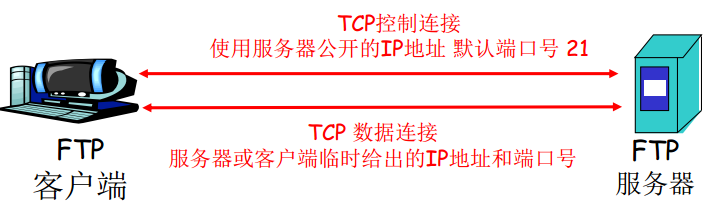
\includegraphics[width=0.6\linewidth]{fig/FTP.png}
\end{figure}

\begin{itemize}
\item 使用FTP协议首先建立\textemph{控制连接},然后建立\textemph{数据连接},客户端再通过控制连接发出命令,通过数据连接得到服务器返回的结果或上传数据给服务器。
\item 控制连接为带外数据(\verb'out of band')
\item FTP服务器会保留状态: 当前目录、已做的认证
\end{itemize}

如下例,得到IP地址(\verb'202.116.86.101')后,计算端口号(12*256+26=3098),\\
进而建立数据连接\verb'telnet 202.116.86.101 3098'
\begin{lstlisting}
telnet 202.116.86.101 21
220 Microsoft FTP Service
user net
331 Password required for user.
pass 123456
230 User user logged in.
pasv
227 Entering Passive Mode (202,116,86,101,12,26).
list
125 Data connection already open; Transfer starting.
226 Transfer complete.
quit
221
\end{lstlisting}

\subsection{Email协议}
Email有三个主要组件:
\begin{itemize}
\item 用户代理(user agents)
\item 邮件服务器(mail servers)
\item 简单邮件传送协议(simple mail transfer protocol, SMTP):TCP端口号25
\end{itemize}
\begin{figure}[H]
\centering
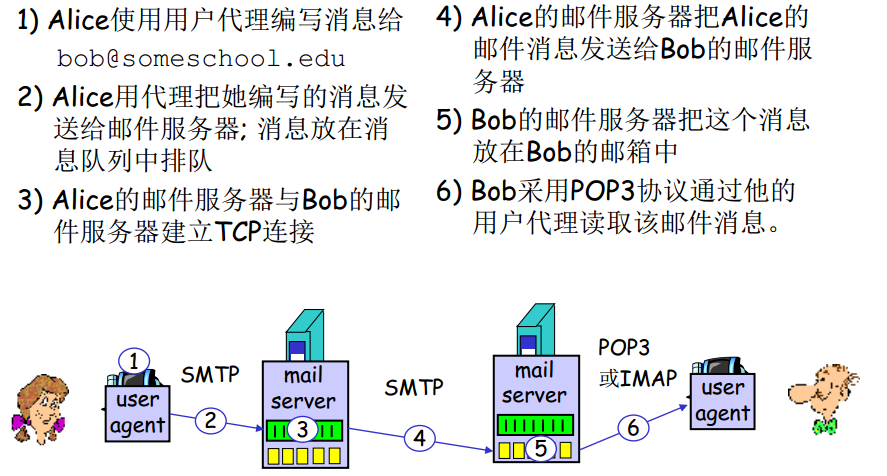
\includegraphics[width=0.7\linewidth]{fig/SMTP.png}
\end{figure}

\subsection{域名系统}
\subsubsection{概述}
域名系统(Domain Name System, DNS)提供的服务
\begin{itemize}
\item 主机名到IP地址的转换
\item 为主机取别名
\item 权威名(Canonical name)、别名(alias names)
\item 为邮件服务器取别名
\item  负载分配(load distribution)
\item 重复的Web服务器: 一个权威名对应一组IP地址
\end{itemize}

\myhline
不采用集中式DNS的原因:不易扩大规模
\begin{itemize}
\item 单点失效
\item 流量过于集中
\item 可能距离数据库太远
\item 维护问题
\end{itemize}

\subsubsection{DNS服务器}
根名字服务器
\begin{itemize}
\item 公开的IP地址,不需要解析名字,由本地名字服务器直接联系
\item 根名字服务器:如果不知道名字映射,把该名字所在的权威名字服务器的IP地址返回给本地名字服务器
\item 根服务器主要用来管理互联网的主目录,全世界只有13台:1个为主根服务器,放置在美国。其余12个均为辅根服务器,其中9个放置在美国,欧洲2个,位于英国和瑞典,亚洲1个,位于日本。
\end{itemize}

权威服务器
\begin{itemize}
\item 顶级域名提供了权威DNS服务器的IP地址,包括com, org, net, edu, uk, fr, ca, jp等
\item 权威DNS服务器:
\begin{itemize}
\item 每个组织机构的公开可访问主机都必须提供公共可访问的DNS记录,这些记录保存在权威DNS服务器上,并把这些主机的主机名映射到IP地址上(e.g., Web, mail).
\item 权威服务器由大型组织或服务提供商维护
\end{itemize}
\end{itemize}

\begin{figure}[H]
    \centering
    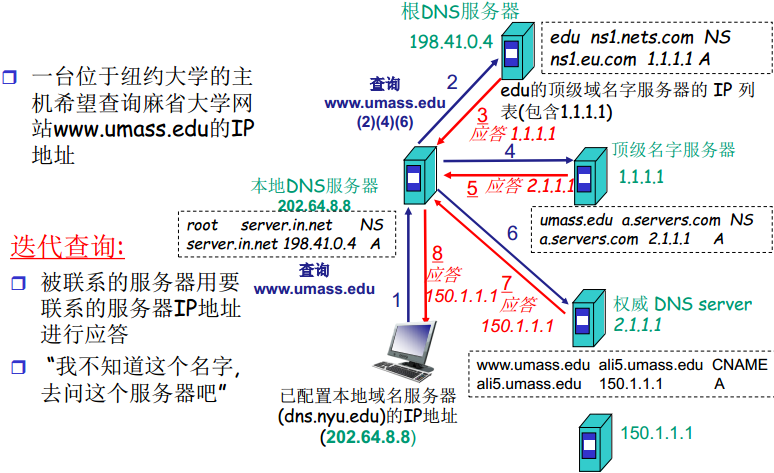
\includegraphics[width=0.8\linewidth]{fig/dns-example.png}
\end{figure}

\subsubsection{资源记录}
采用分布数据库保存资源记录(resource records, RR)
\[\text{(name, value, type, class,ttl)}\]
\begin{itemize}
\item Type=A (Address RR)
\begin{itemize}
\item name是主机名
\item value是IPv4地址
\end{itemize}
\item Type=CNAME
\begin{itemize}
\item name是别名
\item 值是规范名(canonical name)或真名(the real name):
例如, www.jazz.com是主机bp2.jazz.com的别名
\end{itemize}
\end{itemize}

\section{其他内容}
\subsection{无线局域网}
\subsubsection{基本特性}
无线局域网(WiFi)IEEE 802.11
\begin{itemize}
\item 不同标准MAC层一样,改进的是\textemph{物理层}(发、编码、怎么收)
\item 无线信道特点:信号衰减快、抗干扰能力差、发送速率慢、共享信道有限带宽
\end{itemize}
\begin{figure}[H]
    \centering
    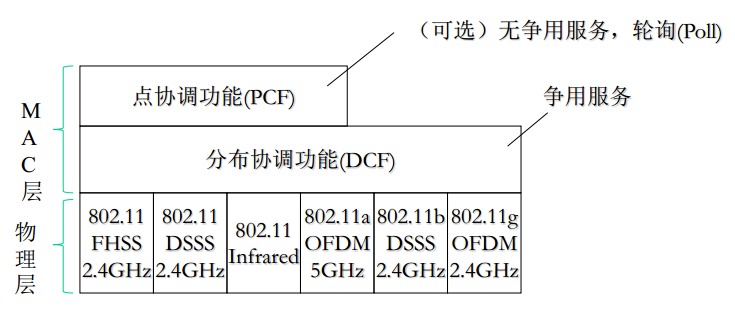
\includegraphics[width=0.6\linewidth]{fig/802-11.png}
\end{figure}

MAC层一般用分布协调功能(DCF)
\begin{itemize}
\item 原子操作:发完数据等待28$\mu$s后才发ACK
\item CSMA/CA(Carrier Avoidance)算法:尽可能少冲突,尽可能少重传;即使空闲也要随机等一段时间
\end{itemize}

\subsubsection{设施}
\begin{itemize}
\item 无固定设施(自组织IBSS):独立基本服务集(Basic Service Set, BSS),不需要路由器,可以几台PC直接连
\item 有固定设施:有个接入点(Access Point, AP),有路由器,连成基本服务集;
扩展的服务集(ESS),完全无缝连接,自动迁移到下一个AP
\end{itemize}

\subsubsection{帧格式}
\begin{figure}[H]
    \centering
    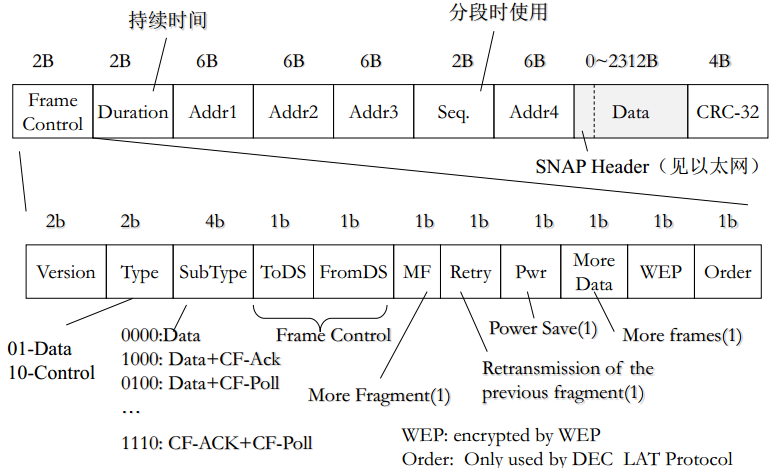
\includegraphics[width=0.8\linewidth]{fig/802-11-frame.png}
\end{figure}

802.11的帧一共有\textemph{4个地址},并没有指出上层协议的部分,所以数据部分(payload)加了\textemph{SNAP}的头部,里面包含了类型指明上层协议。

\begin{figure}[H]
    \centering
    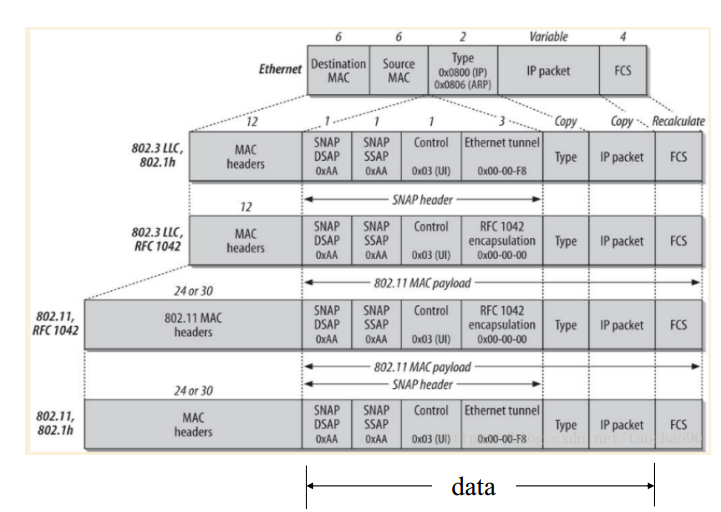
\includegraphics[width=0.8\linewidth]{fig/802-11-frame-2.png}
\end{figure}
\begin{figure}[H]
    \centering
    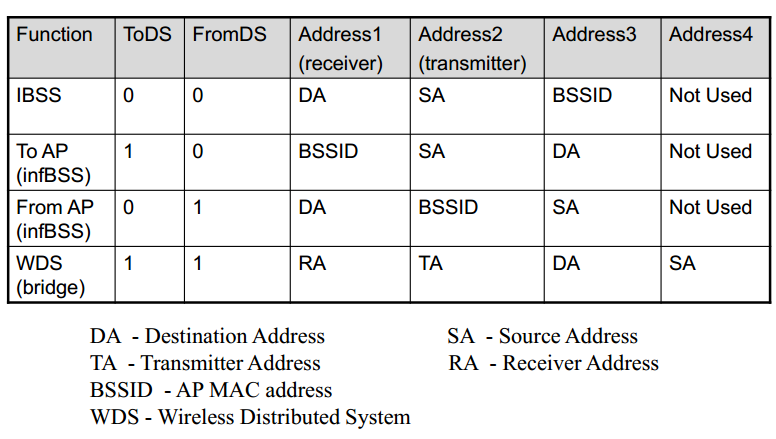
\includegraphics[width=0.8\linewidth]{fig/802-11-frame-3.png}
\end{figure}

\subsubsection{家用小路由器}
\begin{figure}[H]
    \centering
    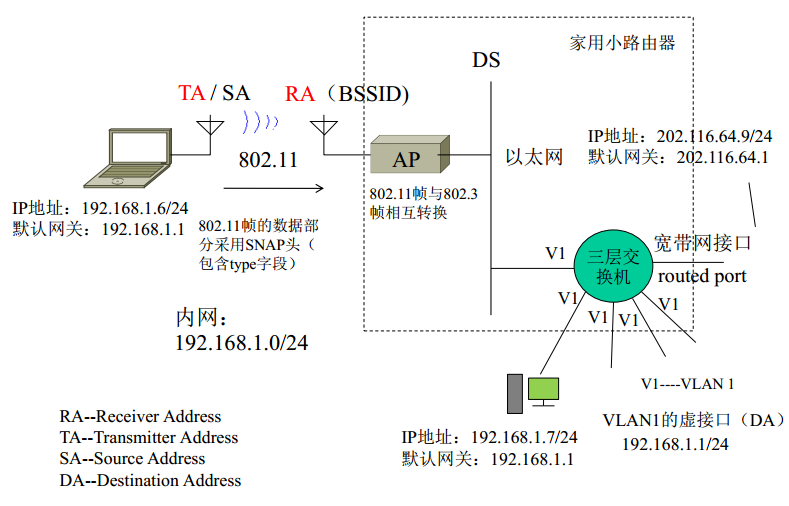
\includegraphics[width=0.8\linewidth]{fig/wlan-example.png}
\end{figure}

\begin{itemize}
\item 很多家用小路由器的内网IP都设成192.168.1.0/24
\item 默认网关配成虚接口的地址(192.168.1.1)
\item 三层交换机的路由表:两个直线网(192.168.1.0/24、202.116.64.9)、默认路由(202.116.64.1),访问因特网就会匹配上默认路由(有线方式)
\item 无线方式:发出来有三个地址
\begin{itemize}
    \item TA(左侧电脑无线网卡的MAC地址)作为SA(源地址)
    \item DA(虚接口的MAC地址)作为目的地址
    \item RA(AP的MAC地址/BSSID),因为有很多个AP,所以要指定RA
\end{itemize}
AP收下帧后,把802.11的帧转化为以太网的帧(有源地址和目的地址了,同时SNAP中也给出了类型),然后用以太网协议发送,三层交换机收到(虚接口地址),再查路由表转发给对应主机或访问外网
\item 当然DA也可以直接写目的主机的IP地址,这样的话交换机就作为透明网桥使用
\end{itemize}

\subsubsection{其他技术}
\begin{itemize}
\item 翻译网桥:一种帧转换为另一种帧
\item 不同频率的WiFi:5GHz WiFi干扰小(不是说现在的5G)
\item 跟以太网不同,WiFi在物理层是有格式的,远距离会换编码,降速进行传输
\item MIMO技术:多发射天线和多接收天线形成多个空间数据流
\end{itemize}

\subsection{网络管理}
SNMP协议:Simple Network Management Protocol

\subsection{广域网}
ADSL不是用语音传,是用数据传的,现在都不用电话线连了。

\subsection{软件定义网络}
软件定义网络(Software Defined Network, SDN):原来路由器交换机都是固定电路,但现在可编程,是未来网络发展方向,最大的好处在于\textemph{虚拟化}。

\begin{center}
\begin{tikzcd}
\text{应用}\arrow{d}\\
\text{控制器}\arrow{d}\\
\text{转发器}
\end{tikzcd}
\end{center}

控制器相当于一个电脑,用来修改下面(几十台)转发器的路由表。

\subsection{多媒体网络}
\begin{itemize}
\item 插值解决丢包问题,因为是连续变化的
\item 传语音数据是用RTP协议传的,基于UDP协议
\item SIP协议用来做网络会议
\item H.232协议则更加完整
\item 令牌桶:没传的时候放令牌,有传的时候用光令牌
\item MPLS加标签实现VPN,沿着同一条路径走过去
\end{itemize}